\documentclass[18pt]{article}
\usepackage[utf8]{inputenc}
\usepackage[a4paper, total={6.5in, 9.5in}]{geometry}
\usepackage{graphicx} % Required for inserting images
\usepackage{enumitem}
\usepackage{booktabs,adjustbox}
\usepackage{multirow,multicol}
\usepackage{xcolor}
\usepackage{array,caption}
\usepackage{amssymb,amsmath}
\usepackage{ragged2e}
\usepackage{tikz,circuitikz}
\usetikzlibrary{shapes,arrows,positioning,patterns,matrix,circuits.logic.IEC, calc}
\usepackage{pgfplots}
\pgfplotsset{compat=newest}
\usepgfplotslibrary{fillbetween,statistics}

% Source : https://tex.stackexchange.com/questions/140567/drawing-karnaughs-maps-in-latex

%isolated term
%#1 - Optional. Space between node and grouping line. Default=0
%#2 - node
%#3 - filling color
\newcommand{\implicantsol}[3][0]{
    \draw[rounded corners=3pt, fill=#3, opacity=0.3] ($(#2.north west)+(135:#1)$) rectangle ($(#2.south east)+(-45:#1)$);
    }


%internal group
%#1 - Optional. Space between node and grouping line. Default=0
%#2 - top left node
%#3 - bottom right node
%#4 - filling color
\newcommand{\implicant}[4][0]{
    \draw[rounded corners=3pt, fill=#4, opacity=0.3] ($(#2.north west)+(135:#1)$) rectangle ($(#3.south east)+(-45:#1)$);
    }

%group lateral borders
%#1 - Optional. Space between node and grouping line. Default=0
%#2 - top left node
%#3 - bottom right node
%#4 - filling color
\newcommand{\implicantcostats}[4][0]{
    \draw[rounded corners=3pt, fill=#4, opacity=0.3] ($(rf.east |- #2.north)+(90:#1)$)-| ($(#2.east)+(0:#1)$) |- ($(rf.east |- #3.south)+(-90:#1)$);
    \draw[rounded corners=3pt, fill=#4, opacity=0.3] ($(cf.west |- #2.north)+(90:#1)$) -| ($(#3.west)+(180:#1)$) |- ($(cf.west |- #3.south)+(-90:#1)$);
}

%group top-bottom borders
%#1 - Optional. Space between node and grouping line. Default=0
%#2 - top left node
%#3 - bottom right node
%#4 - filling color
\newcommand{\implicantdaltbaix}[4][0]{
    \draw[rounded corners=3pt, fill=#4, opacity=0.3] ($(cf.south -| #2.west)+(180:#1)$) |- ($(#2.south)+(-90:#1)$) -| ($(cf.south -| #3.east)+(0:#1)$);
    \draw[rounded corners=3pt, fill=#4, opacity=0.3] ($(rf.north -| #2.west)+(180:#1)$) |- ($(#3.north)+(90:#1)$) -| ($(rf.north -| #3.east)+(0:#1)$);
}

%group corners
%#1 - Optional. Space between node and grouping line. Default=0
%#2 - filling color
\newcommand{\implicantcantons}[2][0]{
    \draw[rounded corners=3pt, opacity=.3] ($(rf.east |- 0.south)+(-90:#1)$) -| ($(0.east |- cf.south)+(0:#1)$);
    \draw[rounded corners=3pt, opacity=.3] ($(rf.east |- 8.north)+(90:#1)$) -| ($(8.east |- rf.north)+(0:#1)$);
    \draw[rounded corners=3pt, opacity=.3] ($(cf.west |- 2.south)+(-90:#1)$) -| ($(2.west |- cf.south)+(180:#1)$);
    \draw[rounded corners=3pt, opacity=.3] ($(cf.west |- 10.north)+(90:#1)$) -| ($(10.west |- rf.north)+(180:#1)$);
    \fill[rounded corners=3pt, fill=#2, opacity=.3] ($(rf.east |- 0.south)+(-90:#1)$) -|  ($(0.east |- cf.south)+(0:#1)$) [sharp corners] ($(rf.east |- 0.south)+(-90:#1)$) |-  ($(0.east |- cf.south)+(0:#1)$) ;
    \fill[rounded corners=3pt, fill=#2, opacity=.3] ($(rf.east |- 8.north)+(90:#1)$) -| ($(8.east |- rf.north)+(0:#1)$) [sharp corners] ($(rf.east |- 8.north)+(90:#1)$) |- ($(8.east |- rf.north)+(0:#1)$) ;
    \fill[rounded corners=3pt, fill=#2, opacity=.3] ($(cf.west |- 2.south)+(-90:#1)$) -| ($(2.west |- cf.south)+(180:#1)$) [sharp corners]($(cf.west |- 2.south)+(-90:#1)$) |- ($(2.west |- cf.south)+(180:#1)$) ;
    \fill[rounded corners=3pt, fill=#2, opacity=.3] ($(cf.west |- 10.north)+(90:#1)$) -| ($(10.west |- rf.north)+(180:#1)$) [sharp corners] ($(cf.west |- 10.north)+(90:#1)$) |- ($(10.west |- rf.north)+(180:#1)$) ;
}

%Empty Karnaugh map 4x4
\newenvironment{Karnaugh}%
{
\begin{tikzpicture}[baseline=(current bounding box.north),scale=0.8]
\draw (0,0) grid (4,4);
\draw (0,4) -- node [pos=0.7,above right,anchor=south west] {RS} node [pos=0.7,below left,anchor=north east] {PG} ++(135:1);
%
\matrix (mapa) [matrix of nodes,
        column sep={0.8cm,between origins},
        row sep={0.8cm,between origins},
        every node/.style={minimum size=0.3mm},
        anchor=8.center,
        ampersand replacement=\&] at (0.5,0.5)
{
                       \& |(c00)| 00         \& |(c01)| 01         \& |(c11)| 11         \& |(c10)| 10         \& |(cf)| \phantom{00} \\
|(r00)| 00             \& |(0)|  \phantom{0} \& |(1)|  \phantom{0} \& |(3)|  \phantom{0} \& |(2)|  \phantom{0} \&                     \\
|(r01)| 01             \& |(4)|  \phantom{0} \& |(5)|  \phantom{0} \& |(7)|  \phantom{0} \& |(6)|  \phantom{0} \&                     \\
|(r11)| 11             \& |(12)| \phantom{0} \& |(13)| \phantom{0} \& |(15)| \phantom{0} \& |(14)| \phantom{0} \&                     \\
|(r10)| 10             \& |(8)|  \phantom{0} \& |(9)|  \phantom{0} \& |(11)| \phantom{0} \& |(10)| \phantom{0} \&                     \\
|(rf) | \phantom{00}   \&                    \&                    \&                    \&                    \&                     \\
};
}%
{
\end{tikzpicture}
}

%Empty Karnaugh map 2x4
\newenvironment{Karnaughvuit}%
{
\begin{tikzpicture}[baseline=(current bounding box.north),scale=0.8]
\draw (0,0) grid (4,2);
\draw (0,2) -- node [pos=1.3,above right,anchor=south west] {$cs_{1}$,$cs_{0}$} node [pos=0.7,below left,anchor=north east] {$cs_{2}$} ++(135:1);
%
\matrix (mapa) [matrix of nodes,
        column sep={0.8cm,between origins},
        row sep={0.8cm,between origins},
        every node/.style={minimum size=0.3mm},
        anchor=4.center,
        ampersand replacement=\&] at (0.5,0.5)
{
                      \& |(c00)| 00         \& |(c01)| 01         \& |(c11)| 11         \& |(c10)| 10         \& |(cf)| \phantom{00} \\
|(r00)| 0             \& |(0)|  \phantom{0} \& |(1)|  \phantom{0} \& |(3)|  \phantom{0} \& |(2)|  \phantom{0} \&                     \\
|(r01)| 1             \& |(4)|  \phantom{0} \& |(5)|  \phantom{0} \& |(7)|  \phantom{0} \& |(6)|  \phantom{0} \&                     \\
|(rf) | \phantom{00}  \&                    \&                    \&                    \&                    \&                     \\
};
}%
{
\end{tikzpicture}
}

%Empty Karnaugh map 2x2
\newenvironment{Karnaughquatre}%
{
\begin{tikzpicture}[baseline=(current bounding box.north),scale=0.8]
\draw (0,0) grid (2,2);
\draw (0,2) -- node [pos=0.7,above right,anchor=south west] {b} node [pos=0.7,below left,anchor=north east] {a} ++(135:1);
%
\matrix (mapa) [matrix of nodes,
        column sep={0.8cm,between origins},
        row sep={0.8cm,between origins},
        every node/.style={minimum size=0.3mm},
        anchor=2.center,
        ampersand replacement=\&] at (0.5,0.5)
{
          \& |(c00)| 0          \& |(c01)| 1  \\
|(r00)| 0 \& |(0)|  \phantom{0} \& |(1)|  \phantom{0} \\
|(r01)| 1 \& |(2)|  \phantom{0} \& |(3)|  \phantom{0} \\
};
}%
{
\end{tikzpicture}
}

%Defines 8 or 16 values (0,1,X)
\newcommand{\contingut}[1]{%
\foreach \x [count=\xi from 0]  in {#1}
     \path (\xi) node {\x};
}

%Places 1 in listed positions
\newcommand{\minterms}[1]{%
    \foreach \x in {#1}
        \path (\x) node {1};
}

%Places 0 in listed positions
\newcommand{\maxterms}[1]{%
    \foreach \x in {#1}
        \path (\x) node {0};
}

%Places X in listed positions
\newcommand{\indeterminats}[1]{%
    \foreach \x in {#1}
        \path (\x) node {X};
}
\graphicspath{ {./Util/} }

% set spacing in tables
\setlength{\tabcolsep}{12pt}
\renewcommand{\arraystretch}{1.5}

\title{
\vspace{10mm}\\
CSE 306\\
Computer Architecture Sessional\\
\vspace{10mm}\\
Assignment-1: 4-bit ALU Simulation\\
\vspace{15mm}\\
Lab Section - A1\\
Group - 06\\
\vspace{5mm}\\
\large{15 December, 2023}\\
\vspace{20mm}
\raggedright
\Large{Members of the Group:\par}
\Large{
\begin{enumerate}[label = \roman*.]
    \item 2005020 - Mostafa Rifat Tazwar
    \item 2005025 - Most. Sonia Khatun
    \item 2005027 - Swastika Pandit
    \item 2005029 - MD. Minhajul Islam Fuad
    \item 2005030 - Fairuz Mubashwera
\end{enumerate}
}
}

\author{}
\date{}

\begin{document}

\maketitle

\newpage
\section{Introduction}
\large
% this portion is for introduction regarding the assignment

The Arithmetic Logic Unit (ALU) serves as the computational core of a computer's central processing unit (CPU). Responsible for executing arithmetic and logic operations, the ALU performs essential tasks such as addition, subtraction,bitwise logical operations, negation and many more. Its speed and versatility make it a vital component in processing instructions efficiently. ALUs come in various architectures, adapting to different computational demands across applications. To understand modern computing devices, knowing about the ALU – its role and design – is vital.
\par
The ALU we designed consisted of three control signals, through which we facilitated six operations: decrement, subtract with borrow, 
subtract, negation, bitwise AND, and XOR operations. The arithmetic unit was responsible for managing the arithmetic operations, while our logical unit executed the 
rest. The control signals supervised the entire ALU operations.
\par
Creating an ALU demands creative thinking from the designer. We employed decoders and multiplexers to link the control signals to our specified operations. Additionally, we repurposed specific ICs to perform operations beyond their intended functions. Our focus was on maximizing the utilization of the resources (ICs) at our disposal, ensuring an optimized design.

\par
We also incorporated 4 status flags , Carry(C), Sign(S), Overflow(V) and Zero(Z) flags, in our design. These flags followed the rules of Assembly Language with some flexibility. They imply :
\vspace{5mm}

\begin{enumerate}[label=\alph*)]
    \item \textbf{C} :- C or Carry Flag is the carry out $C_{out}$ of the adder in the ALU. It depends on the carry output of arithmetic operations. It is reset during logical operations.
    \vspace{3mm}
    \item \textbf{S} :- S or the Sign bit is the MSB of the output, $O_{3}$.
    \vspace{3mm}
    
    \item \textbf{V} :- V is the overflow flag. If the output of an n-bit ALU exceeds the range of $-2^{n-1} $ to $ 2^{n-1}-1$ then an overflow has occured. V is set when the addition of two positive numbers gives negative output and vice-versa. It is always reset during logical operations.
    $$O_{3} = X_{3} \oplus  Y_{3} \oplus  C_{3} $$
    $$\Rightarrow O_{3} \oplus C_{3} \oplus O_{3} = X_{3} \oplus  Y_{3} \oplus  C_{3}  \oplus C_{3}  \oplus O_{3} $$
    
    \begin{equation}
    C_{3} = X_{3} \oplus Y_{3} \oplus O_{3}
    \label{eq:equation1}
\end{equation}

\begin{equation}
    V = C_{3} \oplus C_{\text{out}}
    \label{eq:equation2}
\end{equation}
    
    $$\therefore V = X_{3} \oplus  Y_{3} \oplus  O_{3}  \oplus C_{out}  $$

where $C_{out}$ is the output carry, $O_{3}$ is the MSB of the output, $X_{3}$ and $Y_{3}$ are the MSB of the first and second input of the adder respectively.
    
    \vspace{3mm}
    \item \textbf{Z} :- Z is the Zero flag, which is set when the output of the ALU is zero and reset otherwise.$$Z = \overline{
    O_{3} \lor  O_{2} \lor  O_{1} \lor  O_{0} 
    }$$
\end{enumerate}







\normalsize
\newpage
\section{Problem Specification with Assigned Instructions}

\large
Design a 4-bit ALU with three selection bits $cs_{2}$ , 
$cs_{1}$ and $cs_{0}$ for performing the following 
operations: \par
\normalsize

\vspace{7mm}
\begin{table}[!h]
    \captionsetup{font=Large}
    \centering
    \begin{tabular}{||c|c|c|c|c||}
    \hline
    \multicolumn{3}{||c|}{\textbf{Control Signals}} & \multirow{2}{*}{\textbf{Function}} &  \multirow{2}{*}{\textbf{Description}} \\ \cline{1-3}
     $cs_{2}$ & $cs_{1}$ & $cs_{0}$ & &\\ \hline
     \hline
     0 & X & 0 & Decrement A & A - 1 \\ \hline
     0 & 0 & 1 & Subtract with borrow & A + $\overline{B}$ (i.e. A - B - 1) \\ \hline
     0 & 1 & 1 & NEG A & $\overline{A}$ + 1\\ \hline
     1 & 0 & 0 & Subtract & A + $\overline{B}$ + 1 (i.e. A - B)\\ \hline
     1 & 0 & 1 & AND & A $\land$ B\\ \hline
     1 & 1 & X & XOR & A $\oplus$ B\\ 
    \hline
    \end{tabular}
    \caption{Problem Specification}
\end{table}



\begin{figure}[!h]
    \captionsetup{font=Large}
    \centering
    \begin{tikzpicture}
    % \draw[white] (0,0) grid (12,10);
    \draw (4,2) rectangle (8,5);
    % text using foreach loop
    \foreach \x/\y/\label in {
        6/3.5/ALU,
        0.5/3.5/Inputs,
        11/3.5/Output,
        5/8/$cs_{2}$,
        6/8/$cs_{1}$,
        7/8/$cs_{0}$,
        2/4.5/A,
        2/2.5/B
    } {
        \node[align=center] at (\x, \y) {\fontsize{17}{20}\selectfont \label};
    }

    \foreach \m/\n/\p/\q in{
        2.5/4.5/4/4.5,
        2.5/2.5/4/2.5,
        8/3.5/10/3.5,
        5/7.5/5/5,
        6/7.5/6/5,
        7/7.5/7/5
    }{
        \draw [-stealth] (\m,\n) -- (\p,\q) ;
    }
    \end{tikzpicture}
    \caption{4-bit ALU}
\end{figure}

\newpage
\section{Detailed Design Steps with K-maps}
\subsection{Design Steps}
\begin{enumerate}[label=\roman*), before=\large]
\item Our design comprises 4 parts: arithmetic unit, logical unit,  selection control, and status flags.
    \item The arithmetic unit computes 4 arithmetic operations (decrement A, subtract with borrow, negate A
and subtract) with the help of a 4-bit parallel adder, basic gates and a multiplexer.
    \item In the adder, the first input is A or $\overline{A}$ which is obtained using 1 XOR IC which complements A when $S_{3}$ is set. The second input is $\overline{B}$ or P which is selected by the multiplexer having $S_{2}$ selection bit. For negate A, A is complemented; A remains unchanged for rest of the operations. For subtract and subtract with borrow operations, $\overline{B}$ is selected, for decrement A, P = 1111 is selected and for negate A operation, P = 0000 is selected.
for Transfer A and c = 1111 for Decrement A.
    \item The adder adds A, $\overline{B}$ with $C_{in}$ = 0 and $C_{in}$ = 1 for
    subtract with borrow and subtract operations respectively. P = 0000, $C_{in}$ = 1 and $\overline{A}$ 
     is used for negate A, so adder outputs $\overline{A}$ + 0 + 1 = -A. During decrement operation,
      P = 1111, $C_{in}$ = 0, that 
      is adder adds 1111 to A which is equivalent 
      to A - 1 + 0 = A - 1.
    \item The logical unit performs 2 logical operations AND, XOR using 1 AND IC, 1 XOR IC, and the output (AND, XOR) of the logical unit is selected by a multiplexer having
selection bit $S_{3}$ (0 for AND,1 for XOR).
    \item The selection control uses the control signals as inputs, an active low decoder, and basic 
gates to output the selection variables, $C_{in}$ and intermediate variable P.
    \item  A third multiplexer selects the final output of the ALU. For selection bit S2 = 0, the output of the logical unit is the final output, and for S2 = 1, the output of the
arithmetic unit is the final output.
    \item The overflow flag, V and carry flag, C is computed from the arithmetic unit. During logical operations, $C_{in}$ = 0 and P = 0000 is selected as the second input of the adder. So there is no chance of overflow and carry, which ensures V = 0 \& C = 0 for logical operations.
    \item Zero flag, Z is computed from the 4 output bits using 3 OR gates and then inverting \newline $O_{3}$ $\lor$ $O_{2}$ $\lor$ $O_{1}$ $\lor$ $O_{0}$ by 1 XOR gate(Z $\oplus$ 1 = $\overline{Z}$).
    \item The sign flag S and carry flag C are obtained from $O_{3}$ and $C_{out}$ respectively.
\end{enumerate}
\newpage
\normalsize
\subsection{K-maps}

\large
\subsubsection{K-map for $S_{3}$}
$S_{3}$ is the selection bit which complements the first input $A_{i}$ using a XOR IC.\par

\begin{figure}[!h]
    \centering
    \begin{Karnaughvuit}
        \maxterms{0,1,2,4,5,6,7}
        \minterms{3}
        \implicantsol{3}{green}
    \end{Karnaughvuit}
\end{figure}
\raggedright
So, there is one minterm. We will be using a decoder (active low output) to implement the minterm.$$S_{3} = \overline{D_{3}}$$

\subsubsection{K-map for $S_{2}$}
$S_{2}$ is the selection bit for the second input of the adder in the arithmetic unit. It chooses either $\overline{B_{i}}$ or $P$. The former is chosen when $S_{2}$ is reset. The later P is chosen when $S_{2}$ is set.
\begin{figure}[!h]
    \center{
    \begin{Karnaughvuit}
        \minterms{0,2,3,5,6,7}
        \maxterms{1,4}
        \implicantsol{1}{green}
        \implicantsol{4}{red}
    \end{Karnaughvuit}
    }
\end{figure}\\
\raggedright
Hence, we get $$S_{2} = D_{4} \land D_{1}$$

\subsubsection{K-map for $S_{1}$}
$S_{1}$ is the selection bit for logical operation.It is set during xor and reset during and operation.
\begin{figure}[!h]
    \center{
    \begin{Karnaughvuit}
        \minterms{0,1,2,3,4,6,7}
        \maxterms{5}
        \implicantsol{5}{green}
    \end{Karnaughvuit}
    }
\end{figure}\\
\raggedright
So the expression is, $$S_{1} = D_{5}$$

\newpage

\subsubsection{K-map for $S_{0}$}
$S_{0}$ is the selection bit for choosing between arithmetic and logical operations. For arithmetic operations, $S_{0}$ is set and reset for the other.
\begin{figure}[!h]
    \center{
    \begin{Karnaughvuit}
        \minterms{0,1,2,3,4}
        \maxterms{5,6,7}
        \implicant{7}{6}{orange}
        \implicant{5}{7}{red}
    \end{Karnaughvuit}
    }
\end{figure}\\
\raggedright
As we are implementing this using active low decoder(using maxterms) we get, $$S_{0} = D_{5}\land D_{6} \land D_{7} $$

\subsubsection{K-map for P}
P is the alternative second input of the adder for arithmetic unit. It will be set during decrement, reset for negation and logical operations.
\begin{figure}[!h]
    \center{
    \begin{Karnaughvuit}
        \minterms{0,1,2,4}
        \maxterms{3,5,6,7}
        \implicant{3}{7}{orange}
        \implicant{7}{6}{yellow}
        \implicant{5}{7}{red}
    \end{Karnaughvuit}
    }
\end{figure}\\
\raggedright
Although the expression is a product of 4 maxterms, we already get AND operation of 3 out of 4 terms using $S_{0}$. Hence, we optimize and get, $$S_{0} = D_{3} \land D_{5}\land D_{6} \land D_{7} = D_{3} \land S_{0} $$

\subsubsection{K-map for $C_{in}$}
$C_{in}$ is the carry input of the adder for arithmetic unit. It will be set only during negation and subtraction.
\begin{figure}[!h]
    \center{
    \begin{Karnaughvuit}
        \minterms{3,4}
        \maxterms{0,1,2,5,6,7}
        \implicantsol{3}{green}
        \implicantsol{4}{red}
    \end{Karnaughvuit}
    }
\end{figure}\\
\raggedright
At this point, we have one gate of OR IC and one of NOT IC remaining in our ALU design. We already have $\overline D_{3}$  from one not gate of that IC. So for optimization, we use \textbf{\textit{De Morgan's law}} and 
get $$C_{in} = \overline{D_{4} \land D_{3}} = 
\overline{D_{4}} \lor \overline{D_{3}} $$ 
\newpage
\section{Truth Table}


\begin{table}[!h]
    \captionsetup{font=large}
    \centering
    \begin{tabular}{||c|c|c|c|c|c|c|c|c|c|c|c||}
    \hline
     $cs_{2}$ & $cs_{1}$ & $cs_{0}$ & $X_{i}$ & $Y_{i}$ & $C_{in}$ & $S_{3}$ & $S_{2}$ & $S_{1}$ & $S_{0}$ & P \\
     \hline
     \hline
     0 & X & 0 & $A_{i}$             & 1            & 0 & 0 & 1 & 1 & 1 & 1 \\ \hline
     0 & 0 & 1 & $A_{i}$             & $\overline{B_{i}}$ & 0 & 0 & 0 & 1 & 1 & 1 \\ \hline
     0 & 1 & 1 & $\overline{A_{i}}$        & 0            & 1 & 1 & 1 & 1 & 1 & 0 \\ \hline
     1 & 0 & 0 & $A_{i}$             & $\overline{B_{i}}$ & 1 & 0 & 0 & 1 & 1 & 1 \\ \hline
     1 & 0 & 1 & $A_{i} \land B_{i}$ & 0            & 0 & 0 & 1 & 0 & 0 & 0 \\ \hline
     1 & 1 & X &   $A_{i}\oplus B_{i}$        & 0            & 0 & 0 & 1 & 1 & 0 & 0 \\ 
    \hline
    \end{tabular}
    \caption{Truth Table for selection bits, intermediate variable and carry input}
\end{table}
\section{Block Diagram}

\begin{figure}[!h]
    \captionsetup{font=Large}
    \centering
    \begin{circuitikz}
    % \draw[green] (0,0) grid (13,13);

    % one not gate
    \draw (-1,7.5) node[not port] (not) {};
    \draw (not.in) -- ++(-1,0) node[left] (a) {$B$};
    \draw (not.out) -- ++(0.3,0) node[right] (y) {};

    % overflow flag
    \draw (10.38,11.85) node[xor port ,scale=1, number inputs=4](XOR1){};

    % zero flag
    \draw (9,10) node[or port, scale=1, number inputs=4, anchor=in 1](OR1){};
    
    % Set the input separation to 0.5 units
    \foreach \i in {1,...,4}{
        \draw (OR1.in \i) ++(-0.5,0) -- ++(0.5,0);
    }
    

    % xor gates
     \foreach \x/\y/\a/\b in {
        0/4/$A$/$B$,
        0/11/$A$/$S_{3}$,
        12.9/9.3/$ $/$1$
    } {
        \draw (\x,\y) node[xor port] (xor) {};
        \draw (xor.in 1) -- ++(-1,0) node[left] (a) {\a};
        \draw (xor.in 2) -- ++(-1,0) node[left] (b) {\b};
        \draw (xor.out) -- ++(0.85,0) node[right] (y) {};
    }

    % and gates
     \foreach \x/\y/\a/\b in {
        0/2/$A$/$B$
    } {
        \draw (\x,\y) node[and port] (and) {};
        \draw (and.in 1) -- ++(-1,0) node[left] (a) {\a};
        \draw (and.in 2) -- ++(-1,0) node[left] (b) {\b};
        \draw (and.out) -- ++(0.85,0) node[right] (y) {};
    }

    % mux
    \foreach \x/\y/\s/\a/\b in 
    {
        1/1/$S_{1}$/$ $/$ $ ,
        1/6.5/$S_{2}$/$ $/$P$, 
        8/3/$S_{0}$/$ $/$ $
    } {
        \draw (\x,\y) -- ++(0,4) -- ++(1,-1) -- ++(0,-2) -- cycle;
        \draw (\x + 0.5,\y + 0.5) -- ++(0,-0.75) node[below] {\s};
        \draw (\x - 1 ,\y + 1) -- ++(1,0) ;
        \draw (\x - 1 ,\y + 3) -- ++(1,0) ;
        \node at (\x -1.5,\y + 1) {\a};
        \node at (\x -1.5,\y + 3) {\b};
        \draw (\x + 1,\y + 2) -- ++(0,1) ;
        \node at (\x+0.5,\y+2) {MUX};
    }   

    % adder
    \foreach \x/\y/\a/\b in 
    {
        4/7.5/$X$/$Y$
    } {
        \draw (\x,\y) -- ++(0,4) -- ++(1.5,0) -- ++(0,-4) -- cycle;
        \draw (\x + 0.75,\y ) -- ++(0,-0.75) node[below] {$C_{in}$};
        \draw (\x + 0.75,\y + 4 ) -- ++(0,1.5) node[above] {$C_{out}$};
        \draw (\x - 1 ,\y + 1) -- ++(1,0) ;
        \draw (\x - 1 ,\y + 3) -- ++(1,0) ;
        \node at (\x - 0.25,\y + 1.25) {\a};
        \node at (\x - 0.25,\y + 3.25) {\b};
        \node at (\x+0.75,\y + 2) {ADDER};
    }

    

    % lines
     \foreach \m/\n/\p/\q in{
        1/11/3/11,
        3/11/3/10.5,
        2/8.5/3/8.5,
        2/3/5/3,
        5/3/5/4,
        5/4/7/4,
        5.5/9.5/7/9.5,
        7/9.5/7/6,
        4.75/13/10/13,
        2.5/8.5/2.5/12.27,
        2.5/12.27/9/12.27,
        3/11/3/11.99,
        3/11.99/9/11.99,
        4.75/11.71/9/11.71,
        7/9.5/7/11.4,
        7/11.43/9/11.43,
        % 5.5/9.5/8.5/9.5,
        8.5/10/8.5/9.15,
        9/5/11/5,
        9.5/5/9.5/8,
        9.5/8/8.5/8,
        8.5/8/8.5/9.2,
        10.75/10.5/9/10.5,
        9/10.5/9/10
    }{
        \draw (\m,\n) -- (\p,\q) ;
    }

    % text
    \foreach \m/\n/\s in{
        10.5/13/$\textbf{C}$,
        2.5/12.5/$X_{3}$,
        3.25/11.75/$Y_{3}$,
        11/11.9/$\textbf{V}$,
        6.75/11.25/$O_{3}$,
        14.1/9.3/$\textbf{Z}$,
        11.25/5/$O$,
        11/10.5/$\textbf{S}$,
        8.25/10/$O_{3}$,
        8.25/9.7/$O_{2}$,
        8.25/9.4/$O_{1}$,
        8.25/9.1/$O_{0}$
    }{
        \node at (\m,\n) {\s}  ;
    }
    
    
    % text using foreach loop
    \end{circuitikz}
    \caption{Block Diagram of ALU}
\end{figure}

\newpage

\begin{figure}[!h]
    \captionsetup{font=Large}
    \centering
    \begin{circuitikz}
    % \draw[green] (0,0) grid (8,8);
    \draw (0,2) rectangle (2,6);

    % lines
     \foreach \m/\n/\p/\q in{
        0/4/-1/4,
        0/3.5/-1/3.5,
        0/4.5/-1/4.5,
        2/4.555/2.4/4.555,
        2/4.925/2.4/4.925,
        2/5.3/2.4/5.3,
        3/4.555/3/6,
        3/6/4.5/6,
        4.5/4.925/5.1/4.925,
        3/3.3/5/3.3,
        5/3.3/5/4.37,
        3/3.7/4/3.7,
        4/3.7/4/2,
        4.6/2/5.3/2,
        4.5/4.1/4.5/2.55,
        3.75/4.1/3.75/0.78,
        3.75/0.78/5.15/0.78,
        3.5/2.9/3.5/0.225,
        3/2.9/3.5/2.9,
        3.5/0.22/5.15/0.22,
        3/4.1/4.5/4.1
    }{
        \draw (\m,\n) -- (\p,\q) ;
    }

    \foreach \y in {0.45,0.65,...,1.05}{
        \draw (2,2 + 2*\y) -- (3,2 + 2*\y);
    }

    \foreach \y in {0,1,...,7}{
        \node at (1.75,2.5 + 0.4*\y) {$D_{\y}$}  ;
    }

     \foreach \m/\n/\s in{
        -1.5/4/$cs_{2}$,
        -1.5/4.5/$cs_{1}$,
        -1.5/3.5/$cs_{0}$,
        5/1.75/$S_{3}$,
        4.5/5.3/$S_{0}$,
        4.75/6/$S_{1}$,
        7.25/4.6/$P$,
        7.2/2.3/$C_{in}$,
        7.5/0.5/$S_{2}$
    }{
        \node at (\m,\n) {\s}  ;
    }

    % 3 input and 
    \draw (3,5.3) node[and port, scale=1, number inputs=3, anchor=in 1](AND1){};
    
    % Set the input separation to 0.5 units
    \foreach \i in {1,...,3}{
        \draw (AND1.in \i) ++(-0.6,0) -- ++(0.6,0);
    }

    % 2 input and
    \draw (6.88,4.645) node[and port] (and2) {};
    \draw (and2.in 1) -- ++(-0.5,0) ;
    \draw (and2.in 2) -- ++(-0.5,0) ;

    \draw (7,0.5) node[and port] (and3) {};
    \draw (and3.in 1) -- ++(-0.5,0) ;
    \draw (and3.in 2) -- ++(-0.5,0) ;
    

    \draw (6.58,2.28) node[or port] (or2) {};

    % 2 not 
    \draw (4.35,2) node[not port,scale=0.5] (not1) {};
    \draw (4.85,2.55) node[not port,scale=0.5] (not2) {};
        
    \end{circuitikz}
    \caption{Selection and Intermediate Variables}
    \label{fig:selection}
\end{figure}


\section{Complete Circuit diagram}

\vspace{5mm}
\begin{figure}[!h]
    \centering
    \captionsetup{font=Large}
    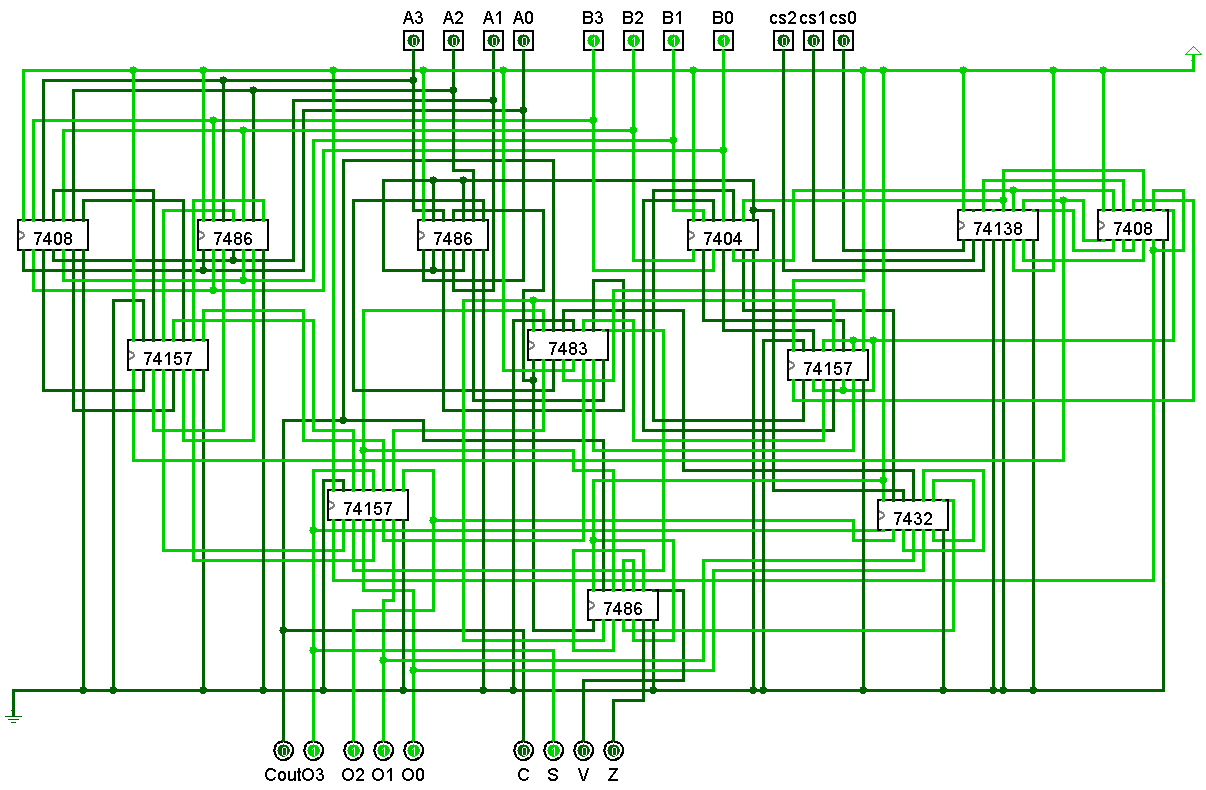
\includegraphics[width=\textwidth]{Util/main.png}
    \caption{Complete ALU circuit}
    \label{fig:enter-label}
\end{figure}
\newpage

\section{ICs used with count as a chart}

\begin{table}[!h]
    \captionsetup{font=Large}
    \centering
    \begin{tabular}{||c|c||}
    \hline
        \textbf{IC} & \textbf{Number of ICs} \\
        \hline
        74138 & 1 \\
        7483 & 1 \\
        74157 & 3 \\
        7432 & 1 \\
        7486 & 3 \\
        7404 & 1 \\
        7408 & 2 \\
    \hline
    \hline
        Total & 12 \\
    \hline
    \end{tabular}
    \caption{ICs and their number}
    \label{tab:ic-number}
\end{table}

\section{The Simulator Used along with the Version Number}

\large

Logisim - 2.7.1

\normalsize

\section{Discussions}
\large
\justifying
The entire project was a pedagogic experience. Several difficulties had to be faced throughout the process.\par 
\vspace{5mm}
Firstly, our circuit design needed a certain degree of creativity. The complement of an input was needed depending on the control signals. So, instead of using a MUX and hex inverter, a XOR IC was used. In addition, an existing selection bit was reused to implement another selection bit. Moreover, techniques like De Morgan's law to simplify and complementing using remaining slot of XOR IC instead of another hex inverter were used. Thus, maximum utilization of the existing ICs were ensured.\par
\vspace{5mm}
Secondly, some difficulties did arise while software simulation using \textbf{Logisim}. 
Changes had to be made in the 7400-lib.circ. 
The $C_{out}$ pin of the IC7483 in the library was faulty. This problem was corrected using a seperate IC7483.circ file in our final ALU software simulation.\par
\vspace{5mm}
Finally, we addressed challenges in the hardware implementation by correcting issues with LEDs, where the use of different types initially caused a power drop. Overheating problems due to connecting LEDs without resistances were resolved through the implementation of proper corrections. Initial misconnections of mini push button switches, providing opposite outcomes, were corrected by the team. The challenge of maintaining a stable power flow across six breadboards was successfully addressed through multiple correction attempts. In debugging the complex circuit, the impracticality of manual methods led us to correct the approach by employing logic design tools for effective resolution.
\newpage

\section{Contribution of Each Member}
\begin{itemize}
    \item 2005020 : Mostafa Rifat Tazwar 
    \begin{itemize}
        \item Circuit design and optimization
        \item Software simulation of ALU circuit
        \item Report writing
    \end{itemize}
    \item 2005025 - Most. Sonia Khatun
    \begin{itemize}
        \item Hardware implementation
    \end{itemize}
    \item 2005027 - Swastika Pandit
    \begin{itemize}
        \item Hardware implementation
    \end{itemize}
    \item 2005029 - MD. Minhajul Islam Fuad
    \begin{itemize}
        \item Hardware implementation
    \end{itemize}
    \item 2005030 - Fairuz Mubashwera
    \begin{itemize}
        \item Hardware implementation
        \item Discussion of report
    \end{itemize}
\end{itemize}

\end{document}